\chapter{Gestión de las Configuraciones}
\label{cap:estadoDelArte}

\section{Introducción}
En este capítulo se presenta el plan de gestión de configuraciones para el sistema de automatización y gestión del Patrocinio Jurídico de la UBA. El objetivo principal es dar a conocer las políticas, estrategias y métodos empleados para mantener la integridad del proyecto, mejorar su desarrollo y garantizar un producto de calidad.


\section{Herramientas para la Administración de Configuraciones}
En esta sección se describen las herramientas y procesos utilizados para gestionar las configuraciones del proyecto. La Tabla~\ref{tabla:gestionConfiguraciones} resume las principales herramientas y sus propósitos.


\begin{table}[h]
  \renewcommand{\arraystretch}{1.5}  % Ajuste del espacio vertical entre filas
  \begin{tabular}{p{0.4\linewidth}p{0.5\linewidth}}
    \toprule
    \textbf{Herramienta/Proceso} & \textbf{Propósito} \\
    \midrule
    Visual Studio Code & Editor de código fuente \\
    GitHub & Control de versiones y gestión de cambios \\
    Jira Software & Administración de tareas y defectos \\
    GitHub Actions & Integración continua \\
    Google Drawio & Creación de diagramas UML \\
    Mockflow  &   Creación de prototipos GUI \\
    Docker & Contenerización de servicios y aplicaciones \\
    Docker Swarm & Orquestación de contenedores \\ 
    Apps Script & Automatización y generación de extensiones para Google Forms \\
    Overleaf & Documentación en Latex \\
    Conda   & Creación de entornos virtuales en desarrollo \\
    Confluence & Documentación y registros internos \\
    \bottomrule
  \end{tabular}
  \caption{Herramientas para la administración de configuraciones}
  \label{tabla:gestionConfiguraciones}
\end{table}


\section{Herramienta de Control de Versiones}

\subsection{Dirección de Acceso}\label{sec:repo-git}
La herramienta de control de versiones utilizada en este proyecto es GitHub. El acceso al repositorio se realiza a través del siguiente enlace:

\href{https://github.com/orgs/proyecto-patrocinio/repositories}{Repositorio}

\subsection{Plan del Esquema de Ramas}
Se establece el siguiente plan para el esquema de ramas:


\begin{figure}[h]
    \centering
    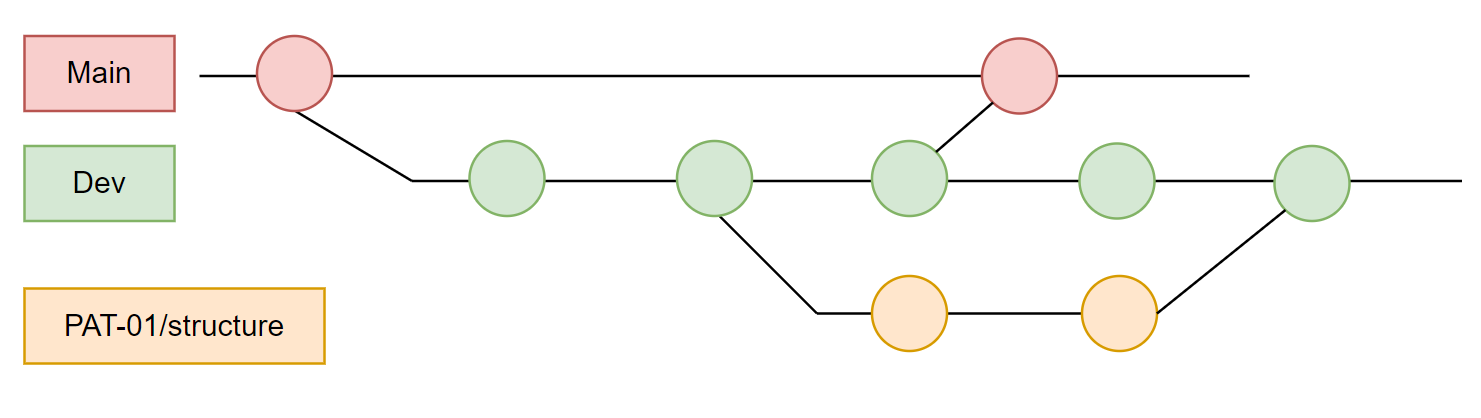
\includegraphics[width=1\linewidth]{fig/branches.png}
    \caption{Ramas de Git}
    \label{fig:enter-label}
\end{figure}


- \textbf{Principal (Main)}: Rama principal del proyecto, refleja la versión estable y funcional del código.
  
- \textbf{Desarrollo (Dev)}: Rama de desarrollo, donde se integran las nuevas características y mejoras.

- \textbf{Funcionalidades (PAT-***)}: Ramas temporales para el desarrollo de características específicas, fusionadas con la rama de desarrollo al completarse.
Esta rama consta del código la issue en Jira seguido de un slash '/' y una breve descripción en inglés. Ejemplo: \textit{PAT-01/structure\_directory}.

Las ramas Feature o funcionalidades utilizan la rama develop como rama primaria. Cuando una feature está terminada, se fusiona con la rama Dev. Las features no deben interactuar nunca directamente con Main.

\subsection{Normas de Etiquetado y de Nombramiento de los Archivos}\label{subsec:semantic_version}

Las versiones se numeran con la siguiente nomenclatura \textbf{MAYOR.MENOR.PATCH} siguiendo el estándar de versionamiento semántico 2.0.0 (Sember) \cite{semver}:
\begin{itemize}
    \item \textbf{PATCH}: Aumenta sólo cuando se corrigen errores o se realiza un refactor que no afecta al funcionamiento, es decir, no realizan cambios en el comportamiento.
    \item \textbf{MENOR}: Se incrementa cuando se añade una nueva funcionalidad compatible con la versión anterior, si algún método se marca como obsoleto debe aumentarse la versión menor.
    \item \textbf{MAYOR}: Se incrementa cuando se produce un cambio que es incompatible con alguna versión anterior, pueden incluir cambios menor y patch.
\end{itemize}


\subsection{Políticas de Fusión de Archivos y Etiquetado en Conformidad con el Progreso de Calidad en los Entregables}

A continuación, se detallan las políticas establecidas para la gestión de versiones y el control de calidad en el proceso de desarrollo de software:

\begin{itemize}
\item \textbf{Control de Versiones en Main:} Únicamente se permitirá la inclusión de versiones en producción en la rama principal (Main).
Se incluirá código debidamente testeado, dejando evidencias de las pruebas realizadas en cada entrega.

\item \textbf{Numeración de Versiones en Releases:} En la fase de release, se generará el tag correspondiente en la rama \texttt{main}, siguiendo la estructura estándar de versionamiento semántico mencionada en la sección \ref{subsec:semantic_version}.

\item \textbf{Etiquetado de Versiones:} Cada versión debe ser etiquetada, proporcionando una referencia clara y accesible para su seguimiento. Este etiquetado permitirá una identificación rápida y precisa de los puntos de lanzamiento.

\item \textbf{Integración con Pruebas:} Únicamente se autorizará la fusión de código que haya superado satisfactoriamente las pruebas correspondientes. Esta medida garantiza la estabilidad y calidad del código integrado en la rama principal.

\item \textbf{Estándar de Commits Semánticos:} Cada commit que se envíe debe cumplir con el estándar de commits semánticos establecido. Este enfoque proporciona una estructura clara y consistente en los mensajes de commit, facilitando la comprensión del historial de cambios.

\end{itemize}


\subsection{Convención de Commits y Merge Request}

Para mantener un estándar, se hace uso de commits semánticos, basados en la Convención de Commits Convencionales 1.0.0 \cite{conventional_commits}. Estos siguen la siguiente estructura:

\texttt{PREFIX(CODE): DESCRIPTION}

\textbf{Ejemplo para commits:}
feat(PAT-05): Add function to search for files

\textbf{Ejemplo para merge request:}
feat[PAT-05]: Add Calendar

Puede ver un ejemplo en el siguiente link \href{https://github.com/proyecto-patrocinio/proyecto-patrocinio/pull/100}{Merge Request}.

A continuación se listan los posibles prefijos:

\begin{itemize}
    \item \texttt{feat}: Una nueva característica para el usuario.
    \item \texttt{fix}: Arregla un bug que afecta al usuario.
    \item \texttt{imp}: Cambios que mejoran el funcionalidades o rendimientos.
    \item \texttt{build}: Cambios en las tareas de despliegue o instalación.
    \item \texttt{docs}: Cambios en la documentación.
    \item \texttt{refactor}: Refactorización del código como cambios de nombre de variables o funciones.
    \item \texttt{test}: Añade tests o refactoriza uno existente.
\end{itemize}



\section{Estructura de Directorios}\label{sec:estr-directory}

El diseño del proyecto se organiza en tres repositorios principales alojados en GitHub, cada uno cumpliendo un rol específico en la implementación y gestión del sistema. A continuación, se detallan estos repositorios junto con sus respectivos enlaces:

\begin{itemize}
    \item \textbf{proyecto-patrocinio} [\href{https://github.com/proyecto-patrocinio}{GitHub-unit}]: Este repositorio alberga tanto el núcleo del proyecto como su interfaz de usuario. Se estructura en carpetas específicas para el backend, frontend y archivos de script destinados a Google App Script.
    
    \item \textbf{cms-deploy} [\href{https://github.com/proyecto-patrocinio/cms-deploy}{GitHub-deploy}]: Este repositorio se centra en la orquestación y configuración del despliegue de la plataforma mediante Docker Swarm. Contiene archivos de composición para Docker, plantillas y configuraciones necesarias para asegurar un despliegue efectivo.
    
    \item \textbf{cms-docs} [\href{https://github.com/proyecto-patrocinio/cms-docs}{GitHub-docs}]: Aquí se encuentra toda la documentación del proyecto. Este repositorio incluye información detallada sobre la arquitectura del sistema, sus componentes, guías de instalación y uso, entre otros documentos esenciales para el desarrollo y mantenimiento del proyecto.

    \item \textbf{cms-test} [\href{https://github.com/proyecto-patrocinio/cms-test}{GitHub-test}]: En este repositorio se encuentran los test de sistema. Éste se utiliza en el proceso de verificación y validación del software para garantizar la calidad del mismo.
\end{itemize}

\subsection{Repositorio \textit{cms-deploy}}\label{subsec:directory-deploy}

El repositorio \textit{cms-deploy} se encarga específicamente de la configuración de despliegue. Incluye archivos de composición para Docker Swarm, plantillas y configuraciones necesarias para garantizar un despliegue eficiente y escalable (ver Figura \ref{fig:deploy-directory}).


En la raíz del directorio, destaca el archivo de composición para Docker Swarm, que define el stack de contenedores. Además, se encuentra la carpeta \texttt{resources}, que contiene archivos de configuración y variables de entorno para los contenedores. La subcarpeta \texttt{templates} dentro de \texttt{resources} se subdivide en dos directorios: \texttt{account} y \texttt{notifications}. El directorio \texttt{account} almacena plantillas HTML relacionadas con los correos electrónicos enviados para el registro de cuentas y cambios de contraseñas. Por otro lado, en el directorio \texttt{notifications}, se encuentran los archivos HTML que se enviarán por correo electrónico para notificar las solicitudes de casos a las comisiones, así como las respuestas a estas solicitudes. 


\begin{figure}[H]
    \centering
    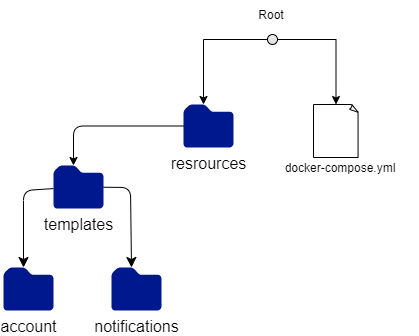
\includegraphics[width=0.5\linewidth]{fig/deploy-directory.png}
    \caption{Estructura de directorios del repositorio \textit{cms-deploy}.}
    \label{fig:deploy-directory}
\end{figure}

\subsection{Repositorio \textit{cms-docs}}

En el repositorio \textit{cms-docs}, se concentra toda la documentación del proyecto. Desde detalles técnicos hasta guías de usuario, este repositorio actúa como una fuente centralizada de información para desarrolladores, administradores y usuarios finales.

\subsection{Repositorio \textit{proyecto-patrocinio}}

El repositorio \textit{proyecto-patrocinio} constituye el núcleo esencial del proyecto, integrando tanto el backend como el frontend, junto con los scripts para Google App Script.

A continuación, se presenta una representación visual de la estructura de directorios específica del repositorio \textit{proyecto-patrocinio}, ofreciendo una visión detallada de la distribución de archivos y carpetas clave para comprender la organización del código y los recursos del proyecto (ver Figura \ref{fig:unit-directory}).

\begin{figure}[h]
    \centering
    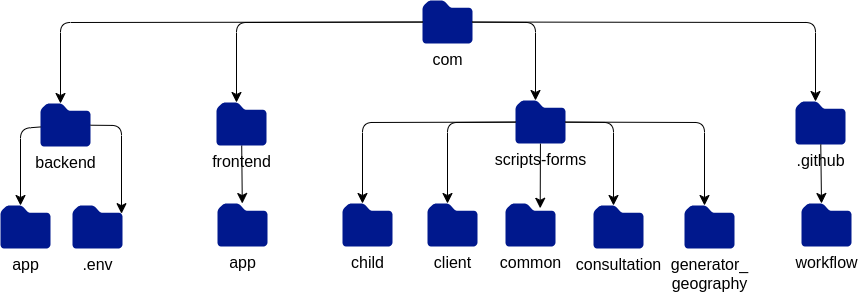
\includegraphics[width=1\linewidth]{fig/directory.png}
    \caption{Estructura de directorios del repositorio \textit{proyecto-patrocinio}.}
    \label{fig:unit-directory}
\end{figure}

Dentro del directorio \texttt{backend}, se encuentran dos carpetas principales: \texttt{.env}, que alberga todas las variables de entorno configurables, y \texttt{app}, donde se desarrolla la API REST en Django. Este último contiene toda la lógica de negocio de la plataforma.

En el directorio \texttt{frontend}, la carpeta \texttt{app} almacena la interfaz de usuario Reactiva, con una mínima lógica necesaria para obtener y visualizar datos.

La carpeta \texttt{scripts-forms} se subdivide en cinco directorios. \texttt{Child} contiene scripts y archivos necesarios para el formulario de registro de un nuevo hijo para un consultante existente. \texttt{Client} incluye scripts y archivos para el formulario de registro de un nuevo consultante. \texttt{Consultation} alberga scripts y archivos para el formulario de creación de una nueva consulta a un consultante existente. La carpeta \texttt{common} contiene archivos compartidos por los formularios mencionados anteriormente. La carpeta \texttt{generator-geography} incluye la hoja de cálculo y scripts necesarios para generar nacionalidades, provincias y localidades en los cuestionarios de los formularios mencionados.

Dentro del directorio \texttt{.github}, la carpeta \texttt{workflows} contiene los pipelines para la integración continua del proyecto. Esta configuración garantiza una gestión eficiente del desarrollo y la implementación continua del proyecto.


\subsection{Repositorio \textit{cms-test}}
En el repositorio \textit{cms-test}, se encuentran todos los casos de prueba automatizados realizados con Robot Framework y Selenium.

\begin{figure}[H]
\centering
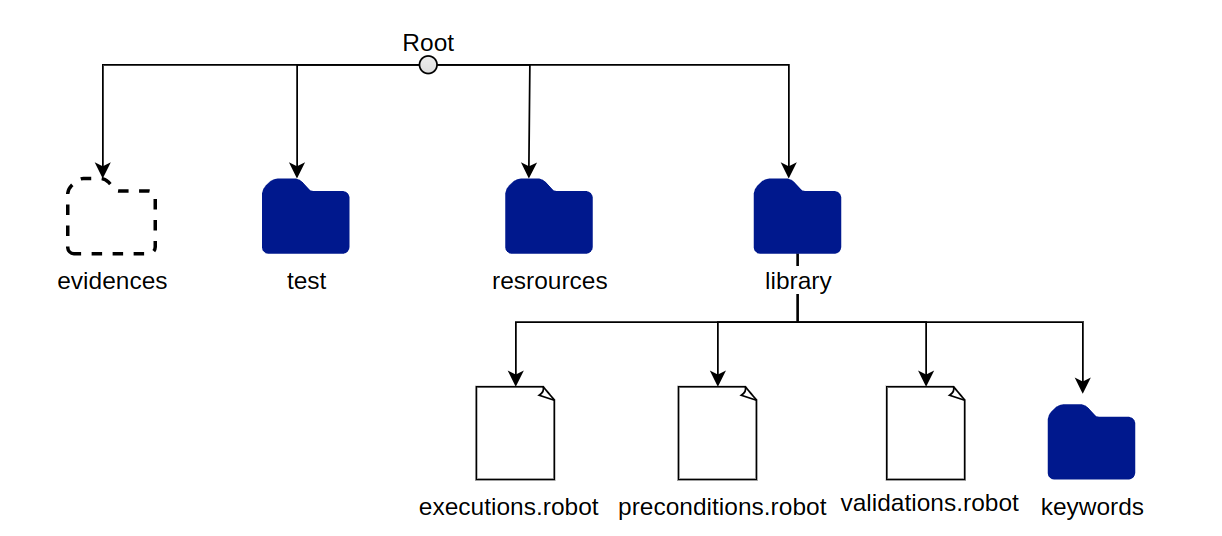
\includegraphics[width=0.9\linewidth]{fig/test-directory.png}
\caption{Estructura del directorio de pruebas en \textit{cms-test}.}
\label{fig:test-directory}
\end{figure}

Dentro del directorio \textit{test}, se ubican los casos de prueba específicos. En el directorio \textit{resources} se almacenan los archivos utilizados en las pruebas. En el directorio \textit{library}, se encuentra la implementación de las \textit{keywords}, divididas en tres archivos: \textit{preconditions.robot}, \textit{executions.robot} y \textit{validations.robot}. Cada archivo contiene las \textit{keywords} relacionadas con las precondiciones (Given), acciones (When) y validaciones (Then) respectivamente, siguiendo la sintaxis de Gherkin \cite{gherkin_docs}.
Por otro lado, en la carpeta \textit{keywords}, se agrupan las \textit{keywords} con la lógica para realizar diversas tareas.

Por último, la carpeta \textit{evidences} se genera automáticamente después de ejecutar los tests, en la cual se recopilan las evidencias generadas para cada caso de prueba.

\section{Herramientas de Gestión de Tareas y Defectos}

Para la supervisión y gestión eficiente de tareas y defectos, se empleó JIRA (\href{https://prietojulii.atlassian.net/jira/software/projects/PAT/boards/1}{Link Jira}). Esta plataforma proporciona tanto el backlog como el board del sprint activo, ofreciendo una vista integral del progreso del proyecto. JIRA no solo facilita la asignación y seguimiento de tareas, sino que también ofrece una interfaz interactiva que simplifica la colaboración y la toma de decisiones. 

\subsection{Confluence}
La integración con Confluence añade un valor adicional al proceso de gestión. Con la capacidad de agregar páginas Markdown directamente al proyecto, se promueve la documentación detallada y la contextualización de las issues. Esto no solo mejora la comprensión de los problemas abordados, sino que también facilita la colaboración al proporcionar un contexto más amplio para la toma de decisiones.

\subsection{Issues}
Cada Issue consta de:
\begin{itemize}
    \item Una descripción detallada.
    \item Un etiquetado que indica el tipo de problema (bug, feat, task).
    \item Un enlace directo a Commits y Merge Request/rama asociados. Para establecer conexiones efectivas entre la Issue, los commits y los Merge Requests o ramas, es esencial agregar el código de la Issue en cada uno de ellos.
    \item Una asignación a persona responsable de hacer avanzar el problema.
    \item Comentarios de cualquier persona con acceso a Jira.
    \item Épica a la cual pertenece.
\end{itemize}
Se ilustra un ejemplo en el siguiente enlace: \href{https://prietojulii.atlassian.net/browse/PAT-44}{Link a la ISSUE}.

\subsection{Épicas}
En el ámbito de la gestión de proyectos, una épica se refiere a una categoría o tema amplio que engloba un conjunto de tareas o historias de usuario relacionadas.
En el contexto de este proyecto, se han identificado diversas épicas que se especifican a continuación.


\subsubsection{Calendario}
Se centra en la integración de calendarios, programación de eventos y cualquier otra característica asociada al seguimiento temporal de los casos.

\subsubsection{Documentación}
Abarca actividades destinadas a mejorar la comprensión y el mantenimiento del proyecto. Incluye la configuración de logs para facilitar la monitorización y depuración del sistema, la actualización regular de los archivos README para proporcionar información actualizada y relevante, el refinamiento y ampliación de las docstrings en el código fuente para mejorar la comprensión de las funciones y métodos, la elaboración de documentación técnica detallada que explique la arquitectura, diseño y decisiones técnicas del proyecto, la creación y actualización de manuales de usuario que guíen a los usuarios finales sobre el uso efectivo del sistema, y la generación de informes detallados que aborden aspectos específicos del proyecto.

\subsubsection{Testing}
Se enfoca en la implementación y mejora de pruebas para garantizar la calidad del software. En este proyecto, la atención se centra principalmente en dos aspectos: pruebas unitarias de backend y frontend, y pruebas de sistema.

\subsubsection{Infraestructura}
Se enfoca en la gestión y mejora de los recursos tecnológicos subyacentes del proyect. Las tareas dentro de esta épica se dividen en dos aspectos clave:

\textbf{Desarrollo de Pipelines:} Se realiza el diseño, desarrollo y optimización de pipelines que automatizan procesos relacionados con la implementación de integración y entrega continua del proyecto.

\textbf{Despliegue en Docker Swarm:} Se establecen y mejoran los procedimientos de despliegue de la aplicación en el entorno Docker Swarm. 



\subsubsection{Notificaciones}
Aborda la implementación de sistemas de notificación eficientes. Esto incluye alertas y correos electrónicos que informe sobre eventos relevantes en el sistema.

\subsubsection{Comentarios}
Se dedica a la implementación de la funcionalidad de comentarios dentro de las consultas, incluyendo la carga de documentos.

\subsubsection{Panel de Control}
Se centra en la creación de las páginas de panel de control, el cual consta de tablas para visualizar los datos y descargarlos.

\subsubsection{Integración con Google Forms}
Busca facilitar la conexión y utilización de formularios de Google dentro del proyecto. Esto implica la automatización de la recopilación de datos y la integración de formularios en procesos específicos.

\subsubsection{Administración}
Se centra en la implementación de la administración básica como el registro de usuarios, gestión de permisos y la carga de datos iniciales al sistema.

\subsubsection{Consultorio}
Abarca las tareas vinculadas a la creación de un tablero de consultoría. Este tablero tiene como objetivo gestionar los casos judiciales y facilitar el proceso de envío de casos a las comisiones correspondientes para su patrocinamiento. Se centra en la implementación de funcionalidades específicas que agilizan y optimizan la administración de casos, desde su registro inicial hasta su asignación a las comisiones pertinentes.

\subsubsection{Tablero}
Engloba las tareas relacionadas con la creación y desarrollo de un tablero destinado a la comisión. Este tablero tiene como objetivo fundamental la gestión integral de casos, incluyendo su ingreso, su seguimiento, y la organización eficiente de cada uno de ellos dentro del sistema. Se enfoca en la implementación de funcionalidades clave que permiten a la comisión llevar a cabo sus responsabilidades de manera efectiva, proporcionando una interfaz intuitiva y completa para la administración de los casos asignados.


\subsubsection{Seguridad y Privacidad}
Se dedica a fortalecer la seguridad y privacidad del sistema. Incluye la implementación de medidas de seguridad, la gestión de accesos y la protección de datos.



\section{Herramienta de Integración Continua}

\textbf{GitHub Actions} es una poderosa plataforma de Integración Continua y Despliegue Continuo (CI/CD) que posibilita la automatización de pipelines para la construcción, prueba y despliegue de proyectos. A través de GitHub Actions, se pueden crear flujos de trabajo personalizables que se encargan de compilar y probar cada pull request enviado al repositorio, así como desplegar las contribuciones fusionadas en la rama principal hacia los entornos de producción.

Un \textbf{WorkFlow} o flujo de trabajo es un proceso automatizado configurable que ejecuta uno o más trabajos (jobs). Estos flujos de trabajo se definen mediante un archivo de configuración YAML que se incorpora al repositorio. La ejecución del flujo de trabajo puede desencadenarse por eventos específicos dentro del repositorio, como cambios en el código, pull requests, o de manera manual.

En el contexto de este proyecto, se han empleado dos flujos de trabajo, uno dedicado al frontend y otro al backend, alojados en el repositorio \textit{proyecto-patrocinio} (ver \ref{sec:estr-directory}).

Para ambos pipelines, se establecen disparadores que inician el flujo de trabajo compuesto por dos etapas principales: \texttt{ci} y \texttt{cd}.

- \textbf{\texttt{triggers}:} La ejecución de los pipelines se configura en respuesta a eventos específicos. Estos eventos incluyen el lanzamiento de una nueva versión (\textit{release}) o la realización de un \textit{push} a las ramas \texttt{main} o \texttt{dev}. En el caso de las ramas \texttt{dev} o \texttt{main}, los pasos del flujo presentan una ligera variación para adecuarse a la gestión de versiones y etiquetas de las imágenes destinadas a Docker Hub.

- \textbf{\texttt{ci}:} Este trabajo realiza un conjunto de pasos esenciales, incluyendo la verificación de la calidad del código, la configuración del entorno de la API, la instalación de dependencias, y la ejecución de pruebas, entre otros. Garantiza que el código enviado cumpla con los estándares definidos antes de proceder con la siguiente etapa.

- \textbf{\texttt{cd}:} La etapa de entrega continua se activa tras el éxito de la etapa de integración continua (\texttt{ci}). En esta fase, se realiza la construcción y la publicación de la imagen de Docker en Docker Hub. La imagen se etiqueta con la versión actual y la etiqueta "latest". Este proceso permite que la imagen esté lista para ser implementada en entornos de producción.



\begin{figure}[H]
    \centering
    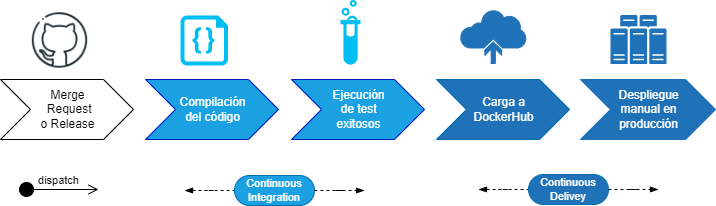
\includegraphics[width=1\linewidth]{fig/cicd.png}
    \caption{CI/CD}
    \label{fig:ci-cd}
\end{figure}

Consulte la sección \href{https://github.com/proyecto-patrocinio/proyecto-patrocinio/actions}{GitHub Actions} del repositorio para ver los detalles de los reportes.




\section{Formato de Entrega}
La entrega del proyecto se realizará vía email adjuntando los siguientes archivos:

\begin{itemize}
    \item Un archivo comprimido denominado \texttt{cms-deploy.zip}, que abarca los componentes esenciales para el despliegue del proyecto.
    \item La documentación en formato PDF.
    \item Un archivo comprimido \texttt{proyecto-patrocinio.zip}, que contiene la unidad del proyecto.
\end{itemize}

Además, se proporcionarán los nombres de las imágenes correspondientes al backend y frontend.




\section{Change Control Board - CCB}

El Comité de Control de Cambios (CCB) se configura como un grupo de partes interesadas (stakeholders) encargadas de supervisar y tomar decisiones relacionadas con propuestas de cambios, requerimientos, hotfixes y otros aspectos inherentes al desarrollo de software. Su objetivo principal es garantizar la coherencia y alineación de estas modificaciones con los objetivos y requisitos establecidos, asegurando la implementación de modificaciones de manera estructurada y controlada.


\subsection{Metodología Ágile}
La elección del marco de trabajo SCRUM se fundamentó en la idoneidad de su enfoque ágil, especialmente en proyectos con requisitos no completamente definidos. SCRUM ofrece una estructura que favorece el progreso incremental a través de sprints y se ajusta bien a la gestión de tareas en entornos dinámicos.

La implementación de SCRUM en este proyecto requirió adaptaciones específicas debido al contexto particular de este proyecto. Se realizaron sprints con una duración flexible de 2 a 4 semanas, ajustando el tiempo según la disponibilidad durante el año lectivo. Adicionalmente, se programaron reuniones de revisión y planificación al final y al inicio de cada sprint, respectivamente, para evaluar avances y definir las metas para el próximo ciclo.

Además, se optó por simplificar los roles de Product Owner, Scrum Master y Developer considerando las limitaciones de recursos de personal.



\subsection{Miembros y Funciones}
A continuación se tabulan los roles de los miembros del proyecto (ver \ref{tab:ccb}).

\begin{table}[h]
    \centering
    \begin{tabular}{|c|p{5cm}|p{4cm}|}
        \hline
        \textbf{Rol} & \textbf{Función} & \textbf{Responsable} \\
        \hline
        Directores del proyecto
        & Revisión del proyecto. Aprobación de decisiones importantes. Gestiona el buen funcionamiento del proyecto, quien controla y administra los recursos (tanto personales como económicos) con el fin de cumplir el plan y el objetivo definido. Se encargan de que todo funcione según lo establecido, resolver desviaciones en el plan, y hacer que los diferentes equipos del proyecto se sincronicen y trabajen juntos.
        & Director, Danilo Paez y Co-directora, Laura Díaz \\
        \hline
        Product Owner
        & Deben conocer perfectamente el producto para garantizar que el equipo de desarrollo cumpla con las expectativas y necesidades.
        & Carina Papini y Melisa Raban \\
        \hline
        Asesor/Consultor
        &  Proporciona asesoramiento y orientación técnica.
        Está disponible para consultas y resolución de dudas
        relacionadas con aspectos específicos del proyecto.
        & Daniel Britos \\
        \hline
        Desarollo Full Stack e Ingeniería
        & Detección y documentación de requerimientos. Diseño y planificación del software en sprints. Encargado de tomar el control de la herramienta de gestión de defecto, documentando específicamente sobre cada problema en el que se trabaja.
        Se encargará de crear un incremento terminado a partir de los elementos del Product Backlog seleccionados por sprint.
        & Julieta Abigail Prieto\\
        \hline
    \end{tabular}
    \caption{Tablero de Miembros y Funciones}
    \label{tab:ccb}
\end{table}

Además, se realiza un reconocimiento especial a Alberto Germán Sotelo y Agustina Cuello por su colaboración como becarios del laboratorio IALAB durante la fase inicial del proyecto realizando tareas de desarrollo backend.

